\section{Concept, Setup \& Implementation}

\subsection{Concept}
To build a functioning prototype, which implements the payment channel described in the previous chapter, the following components are required:
\begin{enumerate}
    \item A supplier in form of a socket
    \item A customer in form of a plug
    \item A server to run a node that connects to the Ethereum blockchain
    \item A Smart Contract on the Ethereum blockchain
\end{enumerate}
All components will communicate with each other over a Wifi connection and TCP.
The following section will summarize all requirements each component of the prototype has to meet. An in depth explanation of the setup and technical implementation will follow in the next section.
\\\\
\textbf{Socket}\\
An AC electrical socket is required. A microcontroller, which can be placed between the electrical circuit and the socket, needs two additional components: a WiFi module to communicate with the web and the plug and a relay to switch the current on and off.
\\\\
\textbf{Plug}\\
An AC electrical plug is required, e.g. a short extension cord, that can be connected to any electronic device. A hall effect-based current meter can be attached to the hot wire to measure the current. This current meter needs to be attached to a microcontroller which also has a WiFi module to communicate with the socket and make http requests to the server.
\\\\
\textbf{Server}\\
The server will run an Ethereum node. This node has to be reachable from the outside, so the microcontrollers can send http requests to it.
\\\\
\textbf{Smart Contract}\\
The Smart Contract acts as a trustee, managing the money during the exchange. It has to be programmed in a way that guarantees that no party can steal from the other.

\newpage
\subsection{Setup}
This section will focus on the technical setup of the hardware components and the installation and setup of all required software.
\\
\subsubsection{Socket}
The Sonoff S20 smart socket was used for the technical implementation of the concept, as it meets all requirements listed in the section above. A microcontroller is automatically powered by the socket it's plugged into. The S20 also has a WiFi module and a relay, which can be switched on and off by said microcontroller. Lastly the microcontroller can be reprogrammed via a serial port.
To program the Sonoff S20, the screws, as seen in the image below, have to be unscrewed first, revealing the logic board with the relay and the serial port.
\\
\begin{figure}[H]
    \includegraphics[width=\textwidth]{img/S20_open.png}
    \caption{Sonoff S20}
    \label{fig:S20}
\end{figure}
\newpage
To program the microcontroller with a computer a FTDI USB to serial converter is required. The converter has to be plugged into the S20 as follows:
\\
\begin{center}
    \begin{tabular} { |c|c| }
        \hline
        FTDI Converter & Sonoff S20 \\
        \hline\hline
        GND & GND \\
        \hline
        TX & RX \\
        \hline
        RX & TX \\
        \hline
        3.3V & 3.3V \\
        \hline
    \end{tabular}
\end{center}
\leavevmode
\\
It's important to notice that the FTDI converter must operate at 3.3V entirely. Caution: some converters only switch the TX and RX pin to 3.3V while the VCC remains at 5V. This can fry the internals of the S20. To program the microcontroller, the button has to be pressed before plugging the pins into the serial port to put it in programming mode. After the pins have been inserted, the button can be released shortly after.
\\
\begin{figure}[H]
    \includegraphics[width=\textwidth]{img/serial_port.png}
    \caption{Serial ports of the Sonoff S20}
    \label{fig:S20_serial}
\end{figure}
\newpage
Both, the socket and the plug, will be programmed using the Arduino IDE. The following steps need to be followed to install the ESP8266 Board, which the S20 is based on:

\begin{itemize}
    \item Inside the Arduino IDE open "Preferences"
    \item Enter \url{http://arduino.esp8266.com/stable/package_esp8266com_index.json} under "Additional Boards Manager URLs"
    \item Open Tools $\rightarrow$ Board $\rightarrow$ Boards Manager
    \item Search and install "esp8266" by "ESP8266 Community"
\end{itemize}

After connecting the FTDI converter to the computer, it should appear under Tools $\rightarrow$ Port. To successfully flash code to the S20 the following settings have to be set:

\begin{itemize}
    \item \textit{Board}: "Generic ESP8266 Module"
    \item \textit{CPU Frequency}: "80 MHz"
    \item \textit{Flash Size}: "1M (no SPIFFS)"
\end{itemize}
\leavevmode

\subsubsection{Plug}
The device to control the measurement of current in the plug and handle the communication with the socket is the Heltec WiFi Kit 8, which is based on an ESP8266 as well and has a 0.91 inch OLED display.
\\
\begin{figure}[H]
    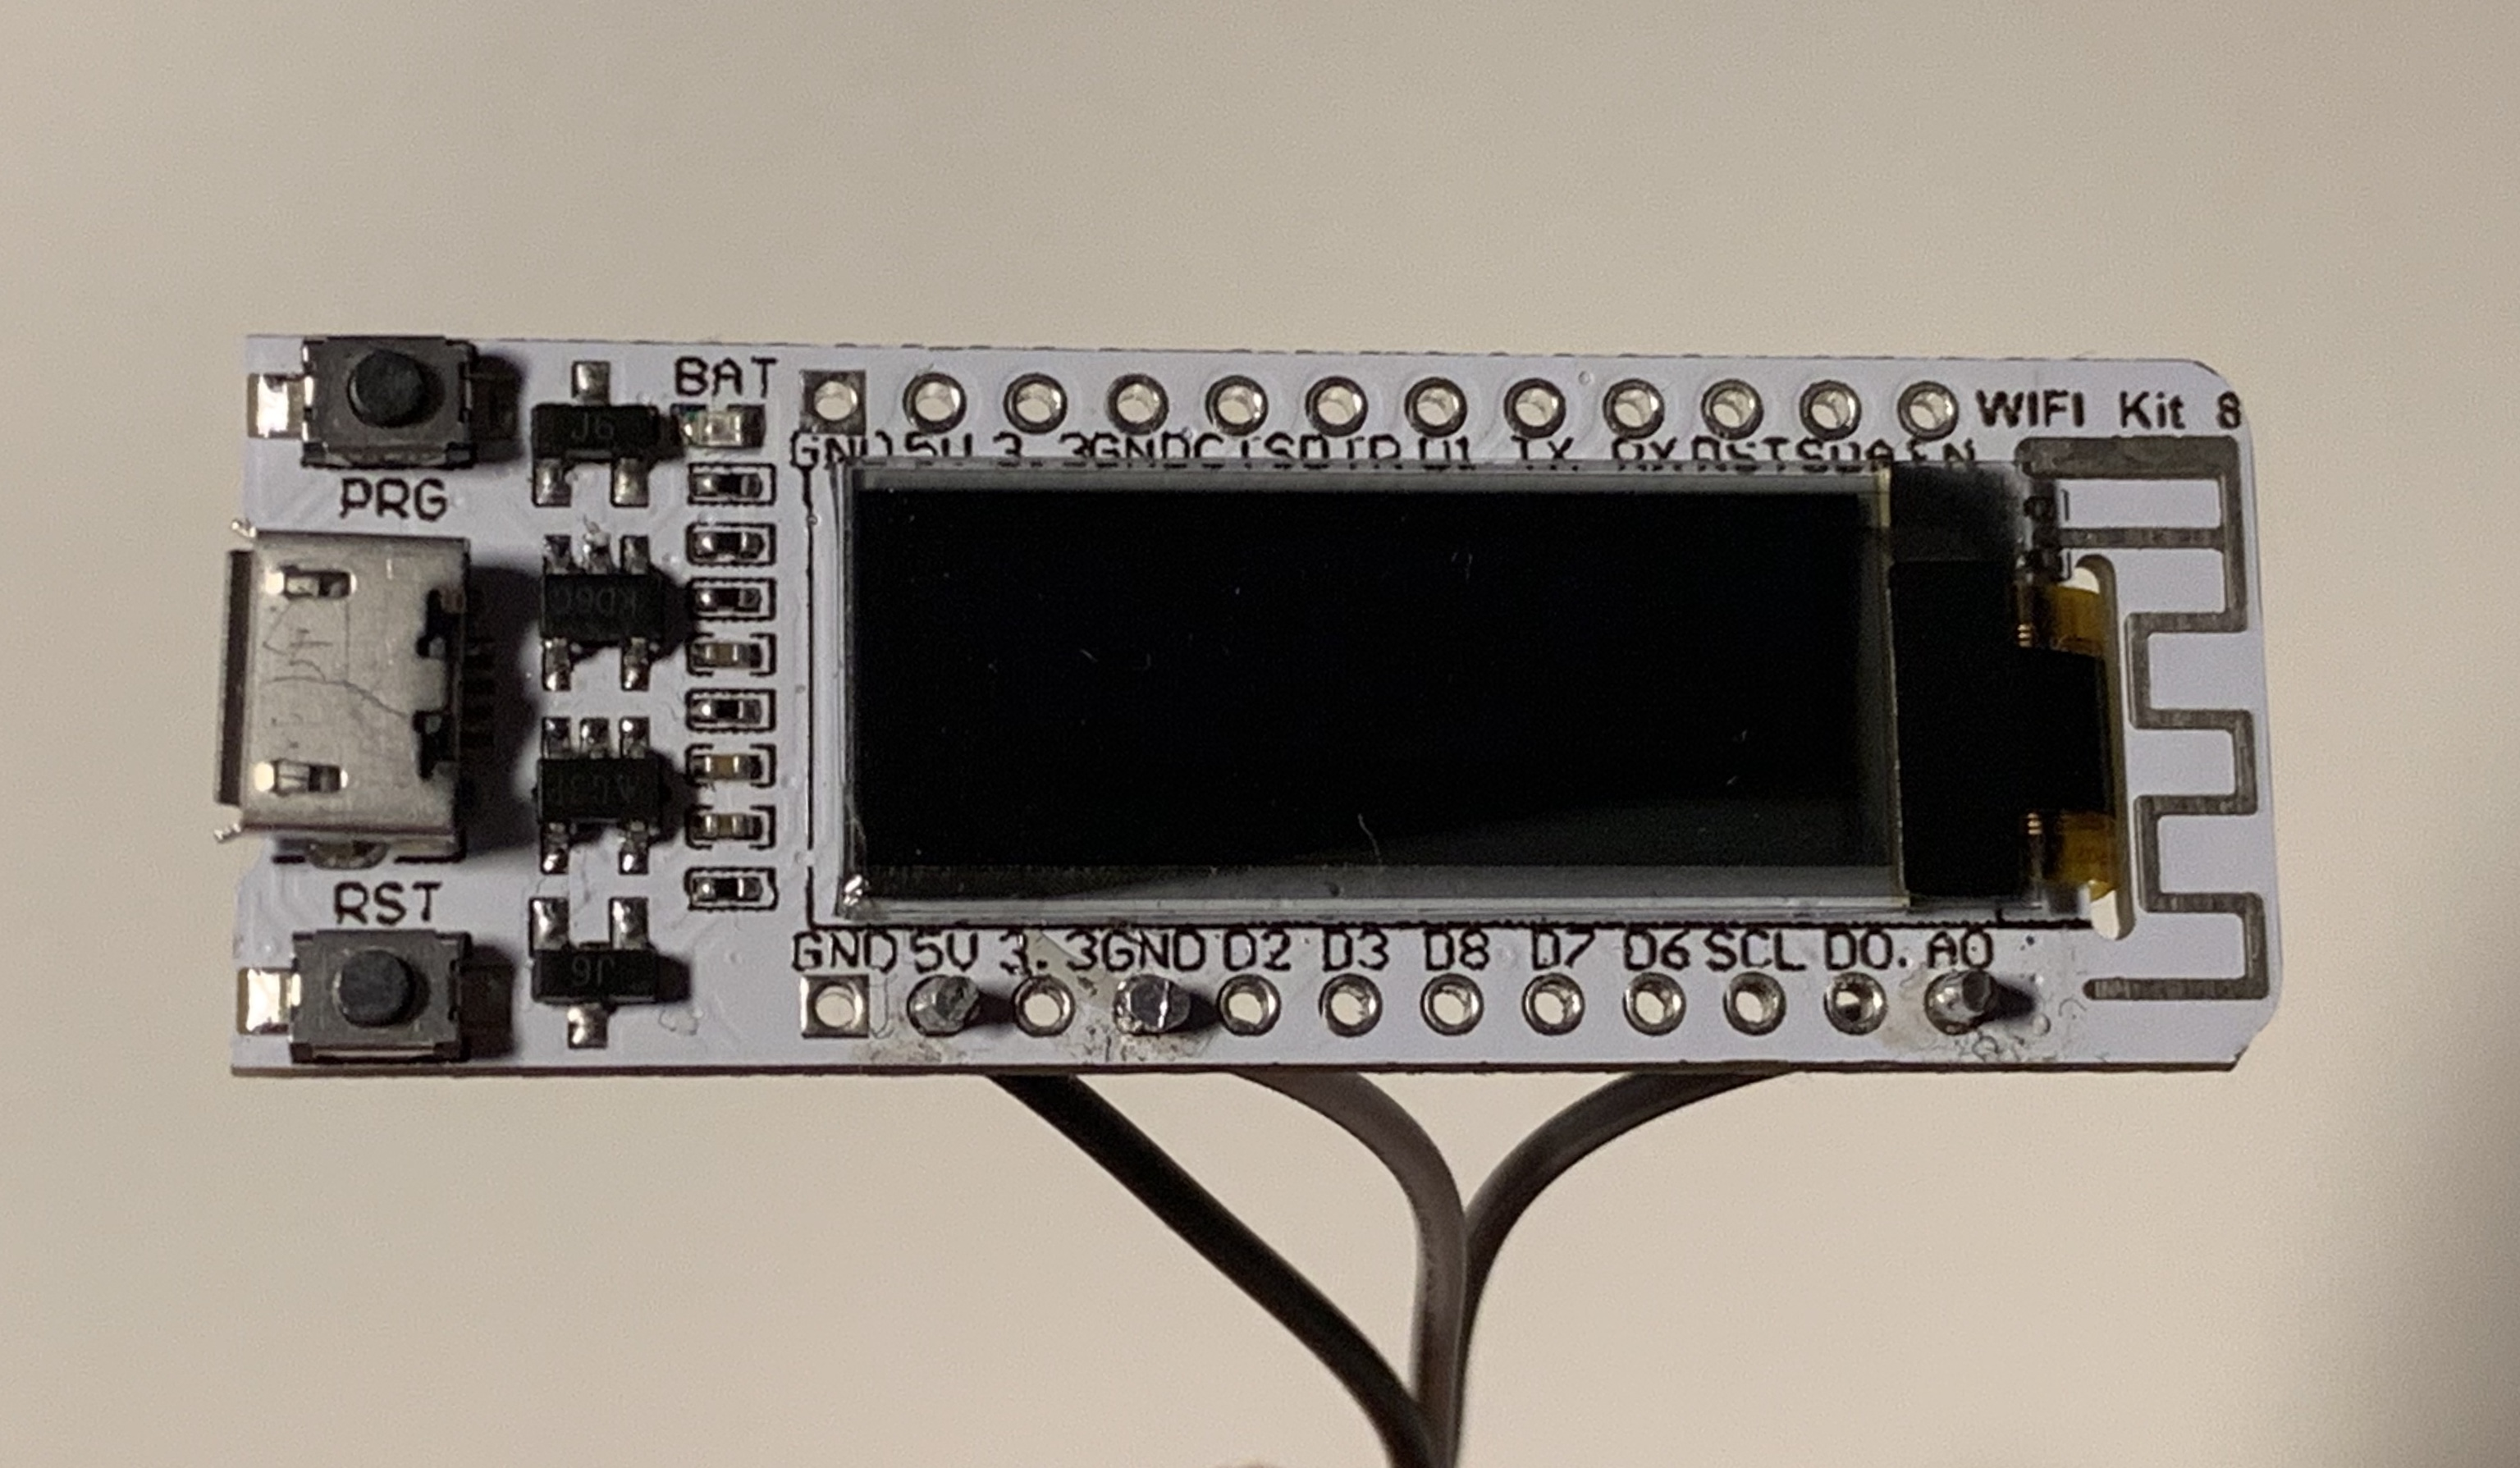
\includegraphics[width=\textwidth]{img/heltec.jpg}
    \caption{Heltec WiFi Kit 8}
    \label{fig:heltec}
\end{figure}

The ACS712 20A current meter is used to measure the current. It's hall effect-based and provides galvanic isolation up to a minimum of 2.1 kV (RMS)\cite{acs712}. To connect the current meter, a part of the hot wire leading to the plug has to be cut and stripped. Both ends have to be inserted into the screw terminal of the ACS712. The current from the plug will now be redirected underneath the hall sensor.
\\
\begin{figure}[H]
    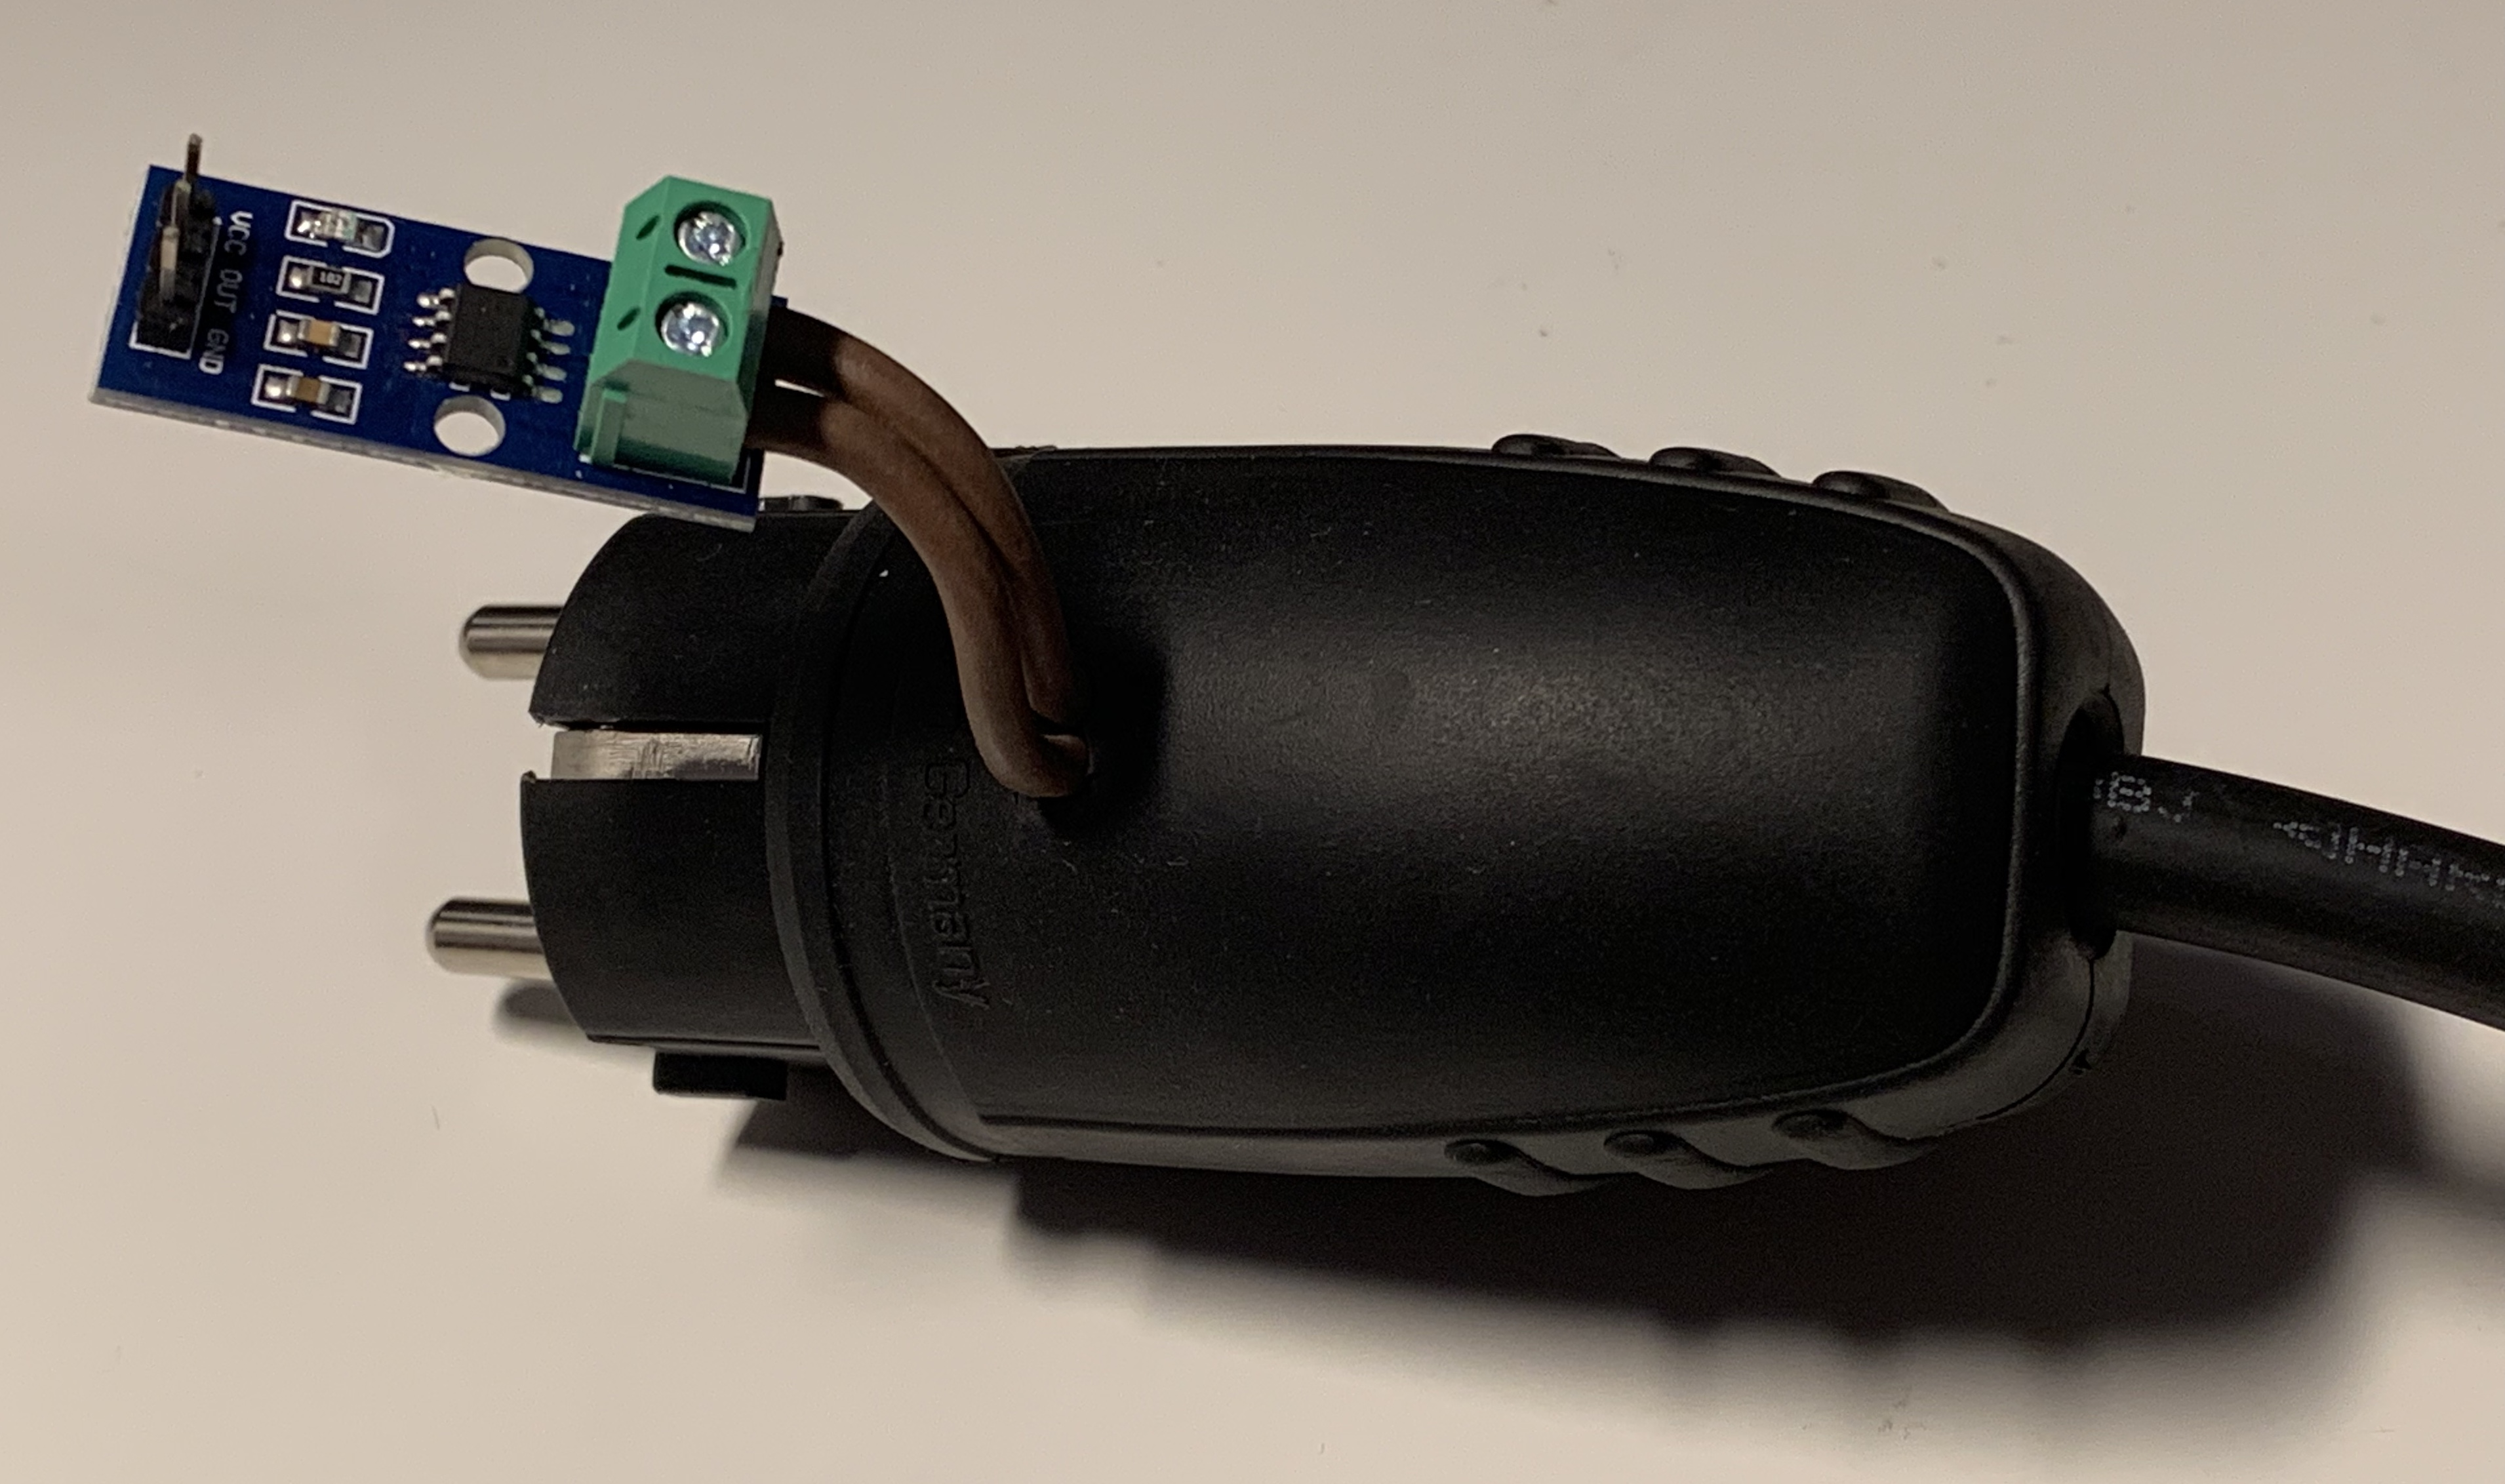
\includegraphics[width=\textwidth]{img/acs712.jpg}
    \caption{ACS712 current meter connected to plug}
    \label{fig:acs712}
\end{figure}

The pins of the current meter have to be soldered to the Heltec board as follows:
\\
\begin{center}
    \begin{tabular} { |c|c| }
        \hline
        ACS712 & Heltec WiFi Kit 8 \\
        \hline\hline
        VCC & 5V \\
        \hline
        OUT & A0 \\
        \hline
        GND & GND \\
        \hline
    \end{tabular}
\end{center}
\leavevmode
\\
To program the Heltec WiFi Kit 8, USB to UART drivers need to be installed first. The download link can be found under "References"\cite{vcp-drivers}. Next, if the ESP8266 was not installed inside the Arduino IDE yet, the instructions found in the section above can be used to install the board.
\\
After a successful driver installation, the board should be found under Tools $\rightarrow$ Port when the device is connected to the computer.
\newpage
The following settings are required to ensure a successful flash of the Heltec WiFi Kit:

\begin{itemize}
    \item \textit{Board}: "NodeMCU 1.0 (ESP-12E Module)"
    \item \textit{CPU Frequency}: "160 MHz"
    \item \textit{Flash Size}: "4M (3M SPIFFS)"
\end{itemize}
\leavevmode

\subsubsection{Libraries}
The prototype relies on some external libraries that have to be installed additionally:
\\\\
\textbf{Display}\\
To use the display of the Heltec WiFi Kit a special library needs to be installed. Under Sketch $\rightarrow$ Include Library $\rightarrow$ Manage Library search for and install the "U8g2" library by "oliver".
\\\\
\textbf{WebSocket server}\\
The communication between the plug and the socket relies on WebSockets. Download the library as a zip file from the git repository\cite{websockets}.
\\
Install it via Sketch $\rightarrow$ Include Library $\rightarrow$ Add .ZIP Library.
\\\\
\textbf{ECDSA Library}\\
Ethereum relies on the Elliptic Curve Digital Signature Algorithm, although there are some differences to the standard implementation of that algorithm, which will be explained later. The zip library is provided with the source code of this prototype and extends the "micro-ecc" library by Kenneth MacKay\cite{micro-ecc}.
\\

\subsubsection{Server}
A server is mandatory to act as a gateway to the Ethereum blockchain. Geth is the official "Golang implementation of the Ethereum protocol"\cite{geth} and is used to run a full node. After the installation it will be used to send transactions and make Smart Contract calls.
\\\\
A \abbr{Virtual Private Server}{VPS} was used for this implementation running Ubuntu 18.04. The server has a six core CPU, 16 GB of RAM, 400GB SSD and 400 MBit/s unlimited traffic. The following instructions can be used to install the program under Ubuntu. For other environments the link to the instructions can be found under "References"\cite{geth-instructions}.
\newpage
To install geth add the repository first:
\begin{lstlisting}[language=bash, numbers=none]
  $ sudo add-apt-repository -y ppa:ethereum/ethereum
\end{lstlisting}

Next, install geth:
\begin{lstlisting}[language=bash, numbers=none]
  $ sudo apt-get update
  $ sudo apt-get install ethereum
\end{lstlisting}
\leavevmode
\\
To interact with the Ethereum Blockchain the entire chain history has to be downloaded first. This can take up to 40 GB of disk space and will take several hours of synchronizing. Geth will be started via this console command:
\begin{lstlisting}[language=bash, showstringspaces=false, numbers=none]
  $ geth console --rinkeby --rpc --rpcapi="db,eth,net,web3,
  personal,txpool" --rpcaddr X.X.X.X --rpcport 8545 --cache=1024
\end{lstlisting}

The launch options have the following purposes\cite{cli-options}:
\begin{itemize}
    \item \textit{rinkeby}: synchronizes the Rinkeby Testnet
    \item \textit{rpc}: enables the HTTP-RPC server, allows to receive JSON RPC requests
    \item \textit{rpcapi}: exposed APIs, listing of all APIs can be found under "References"\cite{json-rpc}\cite{management-apis}
    \item \textit{rpcaddr}: IP address of RPC interface, replace "X.X.X.X" with the IP address of the server, defaults to "localhost". Exposing the RPC interface without any restrictions is not advisable, especially on the Mainnet, as it's a severe security concern.
    \item \textit{rpcport}: listening port of the RPC server
    \item \textit{cache}: memory allocated in MB, a minimum of 1024 MB is advisable for a faster synchronization
\end{itemize}
The console parameter starts a JavaScript console, allowing to interact with the blockchain using the web3 library. Geth currently comes with web3 version 0.20.1\cite{javascript-0.20} but might be upgraded to version 1.0\cite{javascript-1.0} soon. The links to the documentation of both versions can be found under "References".
\\
The version of the web3 library can be checked using:

\begin{lstlisting}[language=bash, numbers=none]
  > web3.version
\end{lstlisting}

The output of the synchronization could hamper the ability to properly read the output of the JavaScript console. The verbosity can be set via the following command:

\begin{lstlisting}[language=bash, numbers=none]
  > debug.verbosity(x)
\end{lstlisting}

Replace x with 0 for silent, 1 for error, 2 for warn, 3 for info, 4 for debug and 5 for detail. The verbosity defaults to info\cite{cli-options}.
\newpage

\begin{lstlisting}[language=bash, numbers=none]
  > eth.blockNumber
\end{lstlisting}

returns the block number of the latest synchronized block, which is the amount of all previous blocks. The first block, the also called the genesis block, starts with the block number 0. The current block number can be checked through so-called block explorers, e.g. {rinkeby.etherscan.io}.
\\
\begin{lstlisting}[language=bash, numbers=none]
  > eth.syncing
\end{lstlisting}
returns the current block number and the highest block number. As soon as the client is synchronized it returns "false"\cite{javascript-0.20}.
\\
\subsubsection{Smart Contract}
\paragraph{Wallet}
The first thing needed to start programming Smart Contracts is an Ethereum wallet. MetaMask is a browser extension for Chrome, Firefox and Opera, that not only allows to manage multiple accounts on multiple test chains, it also injects the web3.js library into websites allowing to interact with the Ethereum blockchain and Smart Contracts on web pages.
Visit the MetaMask\cite{metamask} website and download the browser extension. A new account will be generated using a mnemonic phrase, defined in the BIP39 (Bitcoin improvement proposal)\cite{bip39}. It usually consists of 12 words which represent a private key, essentially creating an easy way to remember / write down private keys. An example for a mnemonic phrase is:
\begin{lstlisting}[language=bash, numbers=none]
  short heavy hidden anger nephew tragic fade dad renew finger among tiny
\end{lstlisting}
This phrase translates to the following seed:
\begin{lstlisting}[language=bash, numbers=none]
  b7b36d9ca1e105045344ecb7ca7b9449bfc0889139c9719876d03cf7b5814861
  37e905b9e94e50c03ca22871937ae3c754dea1427eede8198c6774d90fc1a1f4
\end{lstlisting}

Using the BIP44\cite{bip44} standard an unlimited amount of private keys can be derived from the seed. For example the first private key derived from this seed would be:
\begin{lstlisting}[language=bash, numbers=none]
  0xfb8502c03ea336344dc44b66b1a3c01e2917138e92bfa93c54725166394cd46b
\end{lstlisting}
with the corresponding address
\begin{lstlisting}[language=bash, numbers=none]
  0x4d43c1E254a9333fB0D8A50BD3f01b6787ee8895
\end{lstlisting}
The second derived private key is:
\begin{lstlisting}[language=bash, numbers=none]
  0x64b45c024041178aff2f9ed7b7026fff6890c871818c39c1c7bd826e6aa33773
\end{lstlisting}
\newpage
with the corresponding address
\begin{lstlisting}[language=bash, numbers=none]
  0xd38F7dc2d9B6F6D9d5CB6C8813e213D5DC541458
\end{lstlisting}
and so on. This means that the single mnemonic phrase will act as a backup phrase for all accounts that will be created inside the MetaMask wallet.
After MetaMask was set up create a second account and set the network to Rinkeby.
\\
\paragraph{Getting Ether}
The next step would be to get Ethers on the Rinkeby network to interact with the Blockchain, via the website faucet.rinkeby.io. A public Facebook post or Twitter tweet containing the desired destination address has to be provided to receive the Ethers.
\\
\paragraph{IDE}
The Smart Contract was developed using the Remix. It's an online IDE including a compiler for the language Solidity, various debugging and testing tools and can be found under remix.ethereum.org.
\\
First a compiler has to be set inside the "Compile" tab. Because the programming language was designed especially for Ethereum, it is still under very heavy development with frequent updates coming out. The documentation for each specific version can be found under
\\
\url{https://solidity.readthedocs.io/en/v0.5.8/}
\\
while replacing "0.5.8" (the latest stable version at the time of writing) with the desired compiler version.
\\\\
Inside the "Run" tab the connection to the blockchain can be chosen under "Environment". The most important options are:
\begin{itemize}
    \item \textit{JavaScript VM}: A personal Ethereum blockchain implemented in JavaScript that runs locally. It comes with 5 accounts which are preloaded with 100 Ether. It's suited for early development stages, unit testing, and all in all quick tests, as there are no transaction times.
    \item \textit{Injected Web3}: As mentioned before, MetaMask injects Web3 into websites. When choosing this option, the currently active account and the chosen network in MetaMask are used for development.
\end{itemize}
Underneath, the Smart Contract can be chosen and deployed to the blockchain. Next to the deploy button, constructor arguments can be passed. Optionally an existing Smart Contract can be loaded from an address.
\\\\
After a Contract has been deployed or loaded, all functions and public variables will be listed under the "Deployed Contracts" section. This will be the main way to interact with the Smart Contract.
\\
\paragraph{Solidity}
This paragraph will explain the basics and key features of the Solidity programming language.
A solidity source file has the ".sol" file extension. The language has a C++ style syntax and works very similarly to object-oriented programming and is also called contract-oriented\cite{doc-oriented}. Contracts can be viewed as classes and also work with interfaces and inheritance.
\\
See \ref{lis:sc_basic_ref} for an example of a minimalistic Smart Contract, which demonstrates the general syntax as well as some of the features listed below.
\\\\
\textbf{General notice}\\
There are a few important aspects in how certain things behave during Smart Contract programming and execution:
\begin{itemize}
  \item Solidity does not implement floats at the time of writing. This is especially important for calculations using Ether. Therefore it's important to remember that Ether is always assumed as Wei by Smart Contract functions.
  \item When a function throws, all changes to the state that were made up to this point are reverted and the transaction is marked as failed.
  \item \textit{undefined} and \textit{null} does not exist in Solidity, variables rather have a default type, e.g. 0 for integers\cite{doc-types}.
\end{itemize}
\leavevmode
\\
\textbf{Types}\\
The most important data types in Solidity are\cite{doc-types}:
\begin{itemize}
  \item \textit{bool}: The possible values are "true" and "false".
  \item \textit{integer}: There are signed (\textit{int}) and unsigned (\textit{uint}) integers in Solidity. \textit{uint} is an alias for \textit{uint256}. The smallest size for an integer is 8 bit (e.g. \textit{uint8}), the sizes grow by 8 up to 256 bit. The same applies to signed integers as well.
  \item \textit{address}: The address variable stores 20 bytes.
  \item \textit{address payable}: The address payable variable stores 20 bytes as well. Additionally it holds the members \textit{transfer} and \textit{send} to send Ether to that address.
  \item \textit{bytes32}: Holds 32 bytes of data.
  \item \textit{mapping(keyType $=>$ valueType)}: Mappings work similarly to hash tables. The key can be of any elementary type, the value can be of any type, even another mapping. An example for a frequently used mapping would be the balance variable:
  \\
  \textit{mapping(address $=>$ uint256) balances;}
  \\
  Every address points to a uint256 which represents a balance.
  \item \textit{bytes[]}: Dynamically-sized byte array.
  \item \textit{string}: Dynamically-sized UTF-8 encoded string.
\end{itemize}
\leavevmode
\\
\textbf{Pragma}\\
The first line of a solidity file defines the compiler version\cite{doc-pragma}:
\begin{lstlisting}[language=Solidity, numbers=none]
  pragma solidity ^0.5.4;
\end{lstlisting}
The \^{} symbol means that the code can be compiled by a compiler with the versions 0.5.4 and above, but below 0.6.0. Without the \^{} symbol only the compiler version 0.5.4 can compile the source code.
\\\\
\textbf{Important variables and functions}
Solidity features some global units, variables and functions which can be very useful, if not necessary for Smart Contract programming:
\begin{itemize}
  \item \textit{ether}: The ether unit multiplies the current value by \(10^{18}\), e.g. 3 ether equals 3,000,000,000,000,000,000.
  \item \textit{time units}: The following time units are available: "seconds", "minutes", "hours", "days", "weeks". 1 seconds equals 1, 1 minutes equals 60 seconds or 60, 1 hours equals 60 minutes or 3600 and so on.
  \item \textit{now}: An alias for \textit{block.timestamp}, a \textit{uint256} variable as seconds since unix epoch. The variable is set by the miner during validation so it should not be used for random number generation as the number can be varied by up to $\pm$ 15 seconds, because the timestamp of a block has to be higher than the one of the previous block.
  \item \textit{msg.sender}: Of type \textit{address payable} and contains the sender of the current message. If a function is called directly by an EOA and not by a Smart Contract, \textit{msg.sender} will contain the sender of the transaction.
  \item \textit{msg.value}: Of type \textit{uint256} and contains the number of Wei sent with the current message.
  \item \textit{$<$address payable$>$.transfer(uint256 value)/$<$address payable$>$.send(uint256 value)}: Both functions send "value" in Wei to the payable address. Transfer throws, send returns false on failure.
  \item \textit{function ()}: A function declared without any name is also called the fallback function. This function is called, when no matching function identifier is provided. Usually this function is triggered, when a simple transaction is sent to the Smart Contract, that's why the fallback function can often be seen with the \textit{payable} modifier.
  \item \textit{require(bool condition, string memory message)}: The require function throws if the condition is not met and provides the custom error message.
  \item \textit{keccak256(bytes memory) returns (bytes32)}: Computes the Keccak-256 hash of an input.
  \item \textit{ecrecover(bytes32 hash, uint8 v, bytes32 r, bytes32 s) returns (address)}: For a given message and r, s, v values of a ECDSA signature the function returns the address associated with the public key from the signature.
\end{itemize}
\leavevmode
\textbf{Constructor}\\
A constructor function is optional and can be used to execute code directly when the Smart Contract is written to the blockchain\cite{doc-constructor}.
\\\\
\textbf{Modifiers}\\
A function can have multiple different modifiers, that make it behave in different ways\cite{doc-modifiers}.
First, there is the visibility modifier, which manages the access to functions and variables:
\begin{itemize}
  \item \textit{public}: The public modifier makes a function visible from inside and outside the Smart Contract. Adding the modifier to a variable automatically generates a getter function with the same name as the variable.
  \item \textit{external}: The external modifier is only applicable for functions. It makes them only visible from outside the Smart Contract. To call the function from inside the Smart Contract it has to be called via "this.func()" instead of "func()".
  \item \textit{internal}: The internal modifier makes a function or variable only visible internally. This means they can only be accessed from the contract and all derived contracts.
  \item \textit{private}: The private modifier makes a function or variable only visible from the contract itself. It's important to notice that although a variable might be private, it still can be read, since all data stored on the blockchain is public.
\end{itemize} 
\leavevmode
\\
Reading from the blockchain does not require mining or involve transaction fees. Therefore functions that do not write to storage can be marked as such via a modifier:
\begin{itemize}
  \item \textit{view}: If a function has a view modifier, it cannot write to storage, only read from it.
  \item \textit{pure}: If a function has a pure modifier, it cannot modify storage. Additionally it cannot read state, e.g. read from variables. It's primarily used for computations.
\end{itemize}
\leavevmode
\\
The \textit{payable} modifier allows a function to receive Ether. If Ether is included in a function call that doesn't have the \textit{payable} modifier, it throws.
\\\\
It's also possible to write custom modifiers. The example \ref{lis:sc_basic_ref} will show the function of a custom modifier through a commonly used \textit{onlyOwner} modifier, which only allows the owner of a Smart Contract to call the function.
\\\\
\textbf{Events}\\
Events are an important part of Smart Contract programming for 2 key reasons:
\begin{enumerate}
  \item With a complex Smart Contract handling thousands of transactions, it can get confusing to keep track of all changes made to the state of the Smart Contract. Events are a good way to sort these changes into different categories and make them searchable by specific filters.
  \item Some time passes until a transaction was mined, therefore the return value of a function is not returned to the sender of the transaction. Events can be used to act as a return value. A computer system or a frontend can then scan for these events and act accordingly, e.g. show updates to the user.  
\end{enumerate}
See \ref{lis:sc_basic_ref} for an example of an event.
\\\\
\begin{lstlisting}[language=Solidity, caption={Basic structure of a Smart Contract}, label={lis:sc_basic_ref}]
pragma solidity 0.5.8;

contract ModifierExample{
    // variable to store the owner of the Smart Contract
    address owner;
    // number to demonstrate the view function
    uint256 public num;
    
    // definition of an event
    // the indexed keyword allows to use the parameter as a filter
    event ownerChanged(address indexed oldOwner, address indexed newOwner);
    
    // the constructor gets called after contract creation
    // arguments can be passed to the constructor
    constructor(uint256 _num) public {
        // set owner to the sender of the transaction
        owner = msg.sender;
        // set the number to the passed argument
        num = _num;
    }
    
    // custom modifier
    modifier onlyOwner() {
        // throws if sender of call is unequal to value stored in owner variable
        require(owner == msg.sender, "sender is not owner");
        // _; defines where the code of the function, the modifier is used on, runs
        _;
    }
    
    // function to change the address of the Smart Contract
    function changeOwner(address _owner) external onlyOwner {
        // emits the ownerChanged event
        emit ownerChanged(owner, _owner);
        // sets the owner variable to the passed argument
        owner = _owner;
    }
    
    // the function will execute the code and return the calculated number
    // because of the view modifier no state is modified and no transaction has to be sent
    function calculatedNum() public view returns(uint256) {
        return num * 2;
    }
    
}
\end{lstlisting}

\newpage
\subsection{Implementation}
\subsubsection{Microcontrollers}
\paragraph{Transactions}
As both, the plug and the socket, implement transactions, the following section will explain the generation of on- and off-chain transactions on a microcontroller. The process of sending a transaction, no matter of what kind, can be broken down into the following steps:
\begin{enumerate}
    \item Gather data
    \item Encode data
    \item Hash data
    \item Sign hash
    \item Submit signature
\end{enumerate}
\leavevmode
\\
\textbf{JSON RPC}\\
As previously mentioned, the node was set up to accept and handle http requests, which follow the JSON-RPC 2.0 specification\cite{json-rpc-spec}. The implementation heavily relies on the API, as it is used to not only fetch data from the blockchain, but also to send transactions and make Smart Contract calls\cite{json-rpc}\cite{management-apis}.
\\\\
\textbf{1. Gather Data}\\
The following information is necessary to send an on-chain transaction on the Ethereum Blockchain:
\begin{enumerate}
  \item \textit{to}: Receiving address of the transaction.
  \item \textit{value}: Value of the transaction in Wei.
  \item \textit{data}: Hexadezimal data passed with the transaction.
  \item \textit{nonce}: The \abbr{number used once}{nonce} is important, as it protects a user against replay attacks. The nonce starts at zero and increments by one after a transaction was sent. This means the nonce always equals to the total amount of transactions sent by an account. Without said nonce an attacker could resubmit a transaction, that was already mined, over and over again to drain the balance of a victim.
  \item \textit{gas price}: The fee of a transaction that gets paid out to a miner in Wei. The higher the fee, the faster the transaction will be mined. The RPC-API method "eth\_gasPrice" returns the current gas price. Websites like ethgasstation.info can be used for a more accurate estimation of the gas price, as multiple past blocks are taken into consideration and even average confirmation times for different prices can be estimated. The Rinkeby Testnet uses a \abbr{proof of authority}{POA} mining algorithm, which only allows a few accounts to act as validators, as in a test environment without monetary incentives stability is more important than decentralization. Therefore there are no competing miners and high transaction costs are not really relevant. A transaction with a gas price of 1 GWei will be usually included in the next block resulting in a confirmation time of $<$ 15 seconds.
  \item \textit{gas limit}: The gas limit specifies how much code can be executed with a transaction. The base limit of any transaction, whether it's a Smart Contract call or not, is 21,000 gas – it covers the storage of the transaction on the blockchain as well as the elliptic curve operation to recover the sender of the transaction\cite{design-rationale}. Each additional computational step costs more gas, e.g. an addition (opcode: ADD) costs 3 gas, loading a variable from storage (opcode: SLOAD) costs 200 gas and even goes as far as 20,000 gas if a storage value (variable stored on the blockchain) is set from zero to non-zero. As it can be seen, storing data on the blockchain is one of the most expensive operations to disencourage storing vast amounts of information on-chain. If the gas limit is set too low and there is not enough gas to finish the Smart Contract execution, the transaction is unsuccessful and reverts any changes made. If the limit was set too high, any unused gas is refunded to the sender. Using the "eth\_estimateGas" RPC-API method the gas usage of a Smart Contract call is returned. It's important to note that the node then simulates the Smart Contract call against its own copy of the ledger at the current time. Thus side effects through global variables or different senders can alter the amount of gas that a function requires to execute. The total transaction fee is calculated by multiplying the gas price with the gas limit.
  \item \textit{chain ID}: Each Ethereum Blockchain has a unique chain ID to differentiate different chains. For example the Mainnet uses the ID 1 and the Rinkeby Testnet uses the ID 4. With the Ethereum Improvement Proposal 155 (EIP-155)\cite{eip-155} the chain ID should be included into a transaction to prevent so-called cross chain replay attacks, where a transaction on one Ethereum chain can be resubmitted to another Ethereum chain.
\end{enumerate}
\leavevmode
\\
The off-chain transactions require the following data – the current value of the entire transaction, a nonce and the address of the Smart Contract that is managing the payment channel. The reasoning why these informations were chosen for the off-chain transactions will be explained later in detail.
\\\\
\textbf{2. Encode Data}\\
On-chain transactions are encoded with the \abbr{Recursive Length Prefix}{RLP}\cite{ethereum-yellow-paper}. Before the data listed above can be hashed, it's converted into hexadecimal and therefore byte-arrays. RLP was especially designed for Ethereum to efficiently encode these values with the following rules: 
\begin{itemize}
  \item If a single byte is in the range of 0x00 and 0x7f, the byte is its own encoding.
  \item If a byte array is 0 to 55 bytes long, the byte array is prefixed with a single byte with the value 0x80 plus the length of the byte array.
  \item If a byte array is longer than 55 bytes, its encoded by a first byte that has the value 0xf7 plus the length of the length prefix of the byte array, followed by the bytes describing the length of the byte array and finally the byte array itself.
  \item A list of byte arrays can be encoded as well, as it's required for the transaction data. All items are encoded individually first and then encoded again as a total byte array. This allows to encode data, no matter how nested the information is.
\end{itemize}
For the implementation a RLP C++ library was used, written by Takahiro Okada\cite{rlp-lib}. It had to be modified to make it work for the prototype though:
\begin{itemize}
  \item The library was rewritten, to implement encoding of transactions into one utility library.
  \item The library now supports the EIP-155\cite{eip-155}, when encoding transactions with the chain ID.
  \item A bug was fixed that would incorrectly encode byte arrays that are longer than 55 bytes.
  \item A bug was fixed that would throw an out of memory exception. 
\end{itemize}
The modified library is included with the source code of this bachelor's thesis.
\\\\
Before hashing data in a Smart Contract, which is required for validating off-chain transactions, it has to be encoded in so-called packed mode\cite{packed-spec}. To ensure consistency, the microcontrollers implement the same encoding. The rules are a whole lot simpler than RLP encoding:
\begin{itemize}
  \item all variables are converted to bytes and concatenated together
  \item "types shorter than 32 bytes are neither zero padded nor sign extended"\cite{packed-spec}
  \item "dynamic types are encoded in-place and without the length"\cite{packed-spec}
\end{itemize}
\leavevmode
\\
\textbf{3. Hash data}\\
The encoded data of both, on- and off-chain transactions, is hashed using the Keccak-256 hashing algorithm. The implementation relies on a library that was written by Aleksey Kravchenko and was found in the source code of the firefly DIY hardware wallet\cite{keccak-source}. The library is also included with the source code of this bachelor's thesis.
\\\\
Before signing an Ethereum specific signature, i.e. an off-chain transaction, the data has to be prefixed with an Ethereum specific prefix\cite{prefix}. The data is hashed first, then prefixed according to the following rules:
\\
"\textbackslash x19Ethereum Signed Message:\textbackslash n" + len(message) + message
\\
As a hash is the message that is signed, the length of the prefix will always be 32 bytes. Finally the prefixed message is hashed again. The reasoning behind prefixing a signed message is to protect users unknowingly signing a transaction, when they actually thought they would sign a message.
\\\\
\textbf{4. Sign data}\\
Although Ethereum relies on ECDSA elliptic curve signatures, there are some additional rules and features that differ the signature process from its standard implementation:
\begin{itemize}
  \item It takes up to 2 guesses to recover the public key / address from the $r$ \& $s$ values of an ECDSA signature. Additionally a third value $v$, also called the \textit{recovery ID} is calculated. According to the Ethereum yellow paper\cite{ethereum-yellow-paper} "the recovery identifier is a 1 byte value specifying the parity and finiteness of the coordinates of the curve point for which r is the x-value". Therefore the recovery ID is used to recover the address of the sender from a signature and is determined during the signature process by looking at the y value on the elliptic curve. The recovery ID is determined by the following formula, which is implemented for off-chain transactions:
  \\
  $v = 27 + (y \% 2)$
  \\
  i.e. if y is even the recovery ID equals to 27, if it's odd, it equals to 28. The implementation of the aforementioned EIP-155, which secures transactions against cross-chain replay attacks, is optional and uses the following formula, which is implemented for on-chain transactions:
  \\
  $v = chain\_id * 2 + 35 + (y \% 2)$
  \\
  This means that for transactions on the Rinkeby network the recovery ID is either 43 or 44.
  \item According to the Ethereum yellow paper\cite{ethereum-yellow-paper} the $s$ part of the signature has to be less or equal than half of the numeric value of the elliptic curve $n$, which equals to 
  $0x7FFFFFFFFFFFFFFFFFFFFFFFFFFF
  \\FFFF5D576E7357A4501DDFE92F46681B20A0$
\end{itemize}
As previously mentioned the micro-ecc ECDSA library by Kenneth MacKay was used for the implementation. As the library only covers the standard application of the ECDSA algorithm, the library had to be extended, implementing the Ethereum specific signatures. This extended library is included in the source code of this bachelor’s thesis.
\\\\
\textbf{5. Submit signature}\\
To submit an on-chain transaction, the transaction data and the signature has to be RLP encoded again. The resulting byte array can then be submitted to the Ethereum network using the "eth\_sendRawTransaction" RPC-API method.
\\\\
Both, the plug and the socket, know all transaction data, therefore when the plug is submitting an off-chain transaction, it simply sends the signature to the socket via the WebSockets connection.
\\
\paragraph{State Machine}
The microcontrollers were implemented as finite state machines. The following states with the according IDs were implemented:
\begin{enumerate}[start=0, label=\arabic*:]
  \item disconnected
  \item connected\_P
  \item connected\_S
  \item initialized\_P
  \item initialized\_S
  \item active\_P
  \item active\_S
  \item closed
\end{enumerate}
According to the different states, different code is executed – the suffix \textit{\_P} means that the plug is currently executing code and the socket is expecting a message from the plug, \textit{\_S} means the opposite. The following paragraph will explain the entire payment execution with the help of some flowcharts visualizing the state machine.
\newpage
\begin{figure}[H]
    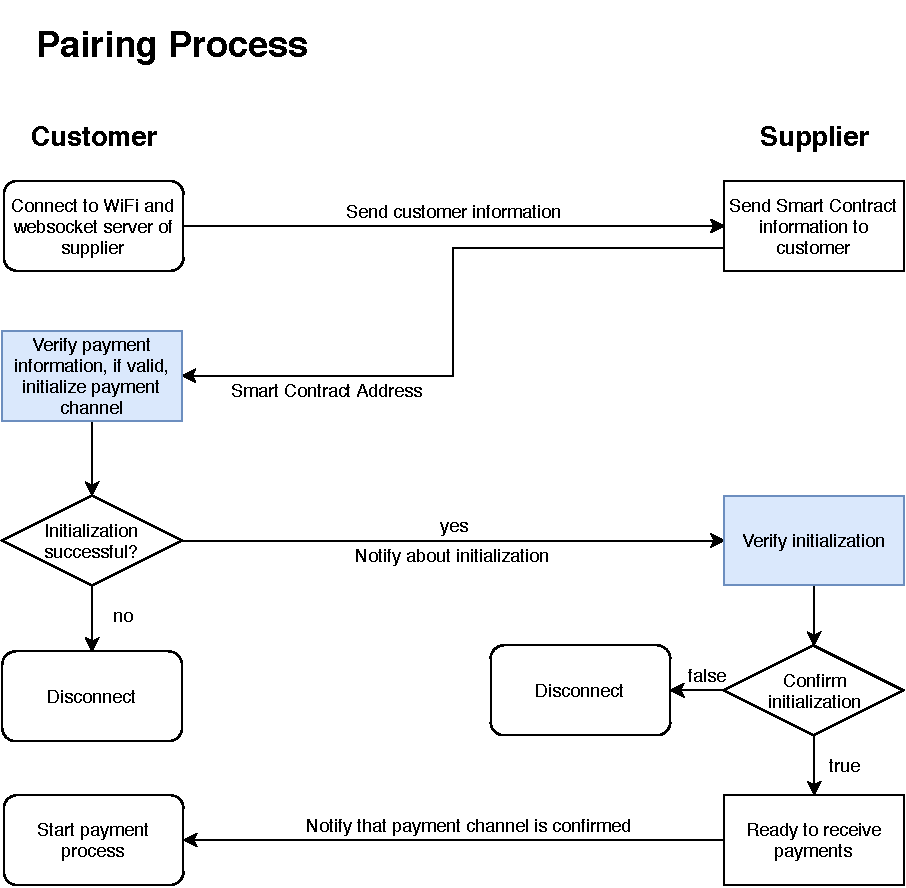
\includegraphics[width=\textwidth]{img/Plug-Socket-pairing_process.pdf}
    \caption{Pairing process}
    \label{fig:pairing_process}
\end{figure}
\begin{enumerate}[start=0, label=\arabic*:]
\item Both, the customer in form of the plug and the supplier in form of the socket start in the \textit{disconnected} state. 
  \item When the plug connects to the websocket server of the supplier, both devices enter the \textit{connected\_P} state. The customer then sends information about itself to the socket in form of its Ethereum address and changes the state to \textit{connected\_S}.
  \item As soon as the socket receives the customer information from the socket, it changes the state to \textit{connected\_S} as well. The supplier can now optionally validate the received data, e.g. check the address against black- or whitelists. If the customer is accepted, the socket sends the address of the Smart Contract, which manages the payment channel, to the plug and changes the state to \textit{initialized\_P}.
  \item As soon as the plug receives the Smart Contract address, it changes the state to \textit{initialized\_P} as well. The customer will now fetch data from the Smart Contract, verify information and initialize the payment channel. These steps will be explained in detail in the next section. If the initialization of the payment channel was successful, the socket is notified and the state is changed to \textit{initialized\_S}.
  \item As soon as the socket receives the notification from the plug, it changes the state to \textit{initialized\_S} and verifies the initialization of the payment channel. Again, the verification will be explained later. If the initialization is confirmed, the socket is ready to receive payments, changes its state to \textit{active\_P} and notifies the plug.
  \item As soon as the plug receives the notification that the socket is ready to receive payments, it changes its state to \textit{active\_P} and the payment process begins.
\end{enumerate}
\leavevmode
\\
\begin{figure}[H]
    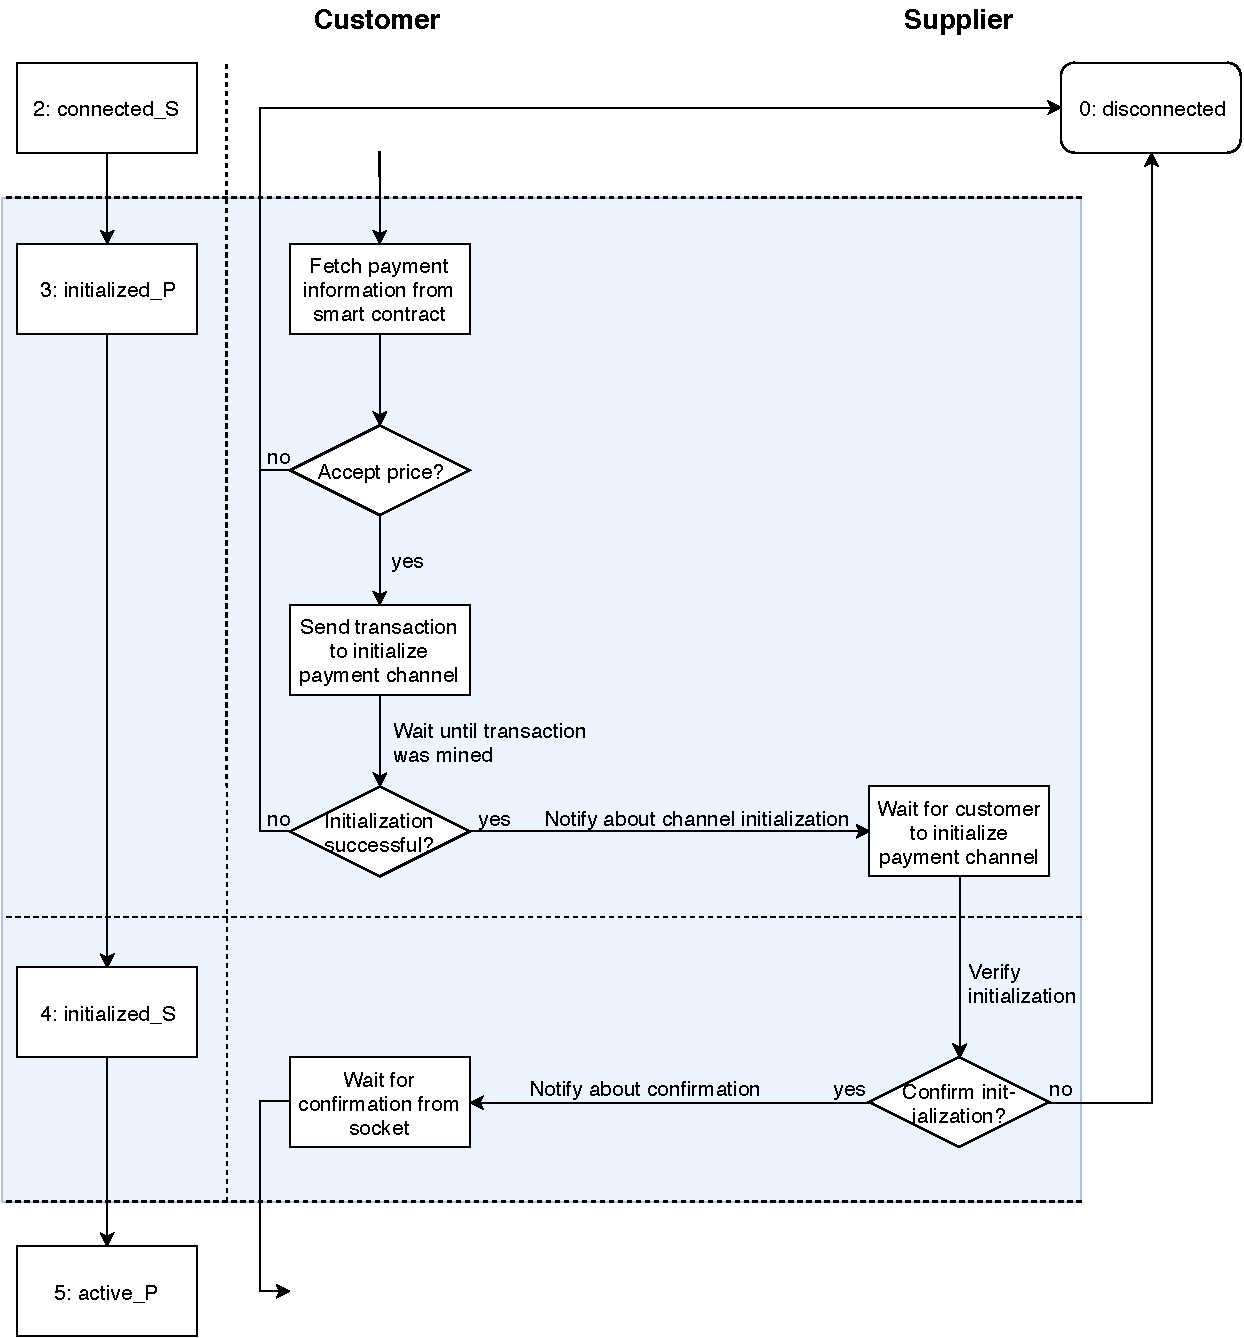
\includegraphics[width=\textwidth]{img/Plug-Socket-verification_process.pdf}
    \caption{Verification process}
    \label{fig:verification_process}
\end{figure}
This section will describe the verification and initialization processes that were skipped in the previous section. The flowchart \ref{fig:verification_process} can be inserted into the blue sections of the flowchart of the pairing process \ref{fig:pairing_process}.
\\\\
\textit{Verification – Customer}\\
The payment information is publicly available on the Smart Contract. After the plug received the address of said Smart Contract, it can fetch all data e.g. the address of the owner (supplier), the price per second, a minimum deposit amount, et cetera. The customer can then either accept or decline the price of the electricity. If the price is accepted, the payment channel can be initialized, through a Smart Contract call. A transaction, containing the maximum value the customer is willing to spend, is sent to the Smart Contract calling the \textit{initializePaymentChannel()} function. The Smart Contract acts as a trustee managing the value and making sure no party can scam the other. After the transaction was sent, the plug has to wait until the transaction was mined, which will take approximately 15 seconds on the Rinkeby Testnet. The RPC-API method "eth\_getTransactionReceipt" can be used to check whether a transaction was mined yet. If the payment channel was set up successfully, the Smart Contract will emit the \textit{InitializedPaymentChannel} event.
\\\\
\textit{Verification – Supplier}\\
After the plug notified the socket about the successful payment channel initialization, the supplier should verify the initialization, e.g. fetch the maximum value of the transaction and make sure the customer address stored on the Smart Contract actually matches the customer address transmitted during \textit{connected\_P}.
\newpage
\begin{figure}[H]
    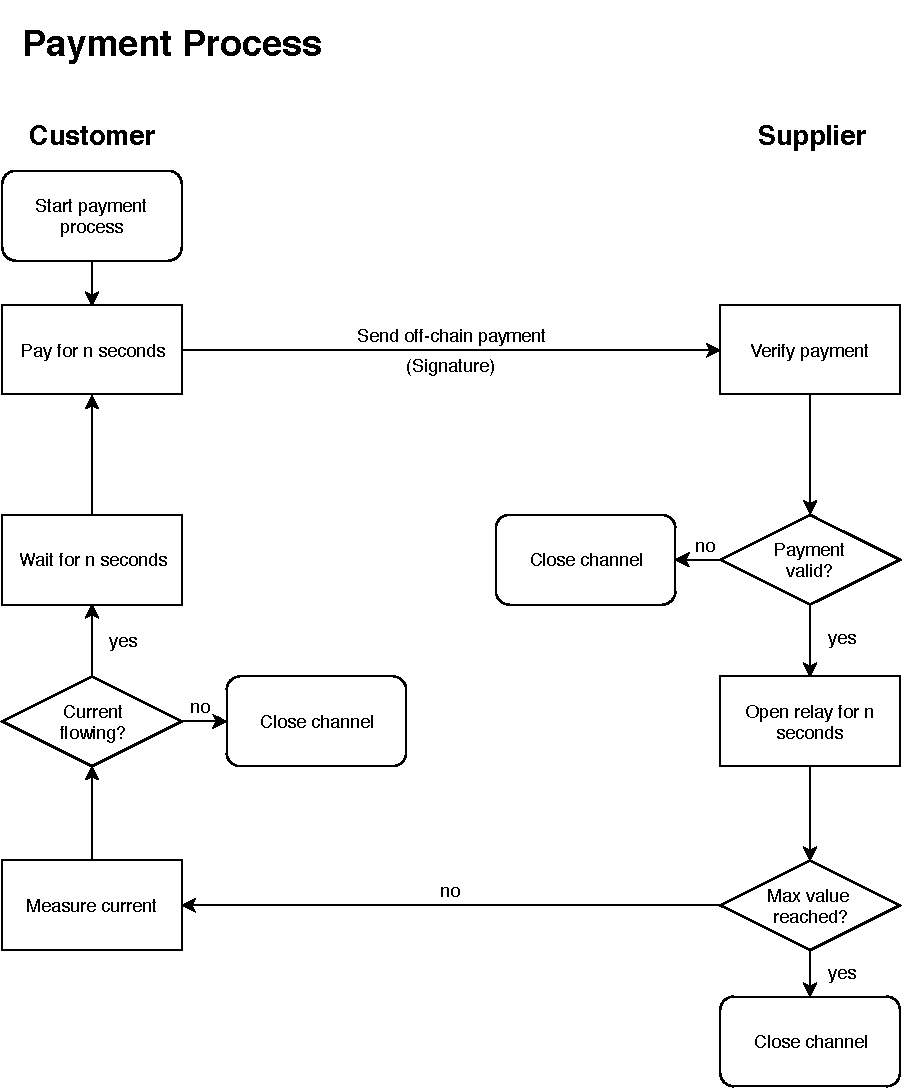
\includegraphics[width=\textwidth]{img/Plug-Socket-payment_process.pdf}
    \caption{Payment process}
    \label{fig:payment_process}
\end{figure}
The payment process starts when the customer sends the first signature, i.e. off-chain transaction to the supplier. The value of the transaction is calculated as follows:
\\
$value = number\_of\_transactions * price\_per\_second * seconds\_between\_transactions$
\\
With the assumed values from chapter 3 (a total price of 18\euro{} over a duration of 11 hours) roughly 0.007\euro{} are transmitted with each off-chain transaction. With the formula above, this means that the value hashed and signed is 0.007\euro{} for the first transaction, 0.014\euro{} for the second, and so on. This means that each time a new transaction is sent it contains the entire value and the last transaction becomes invalid. As the Smart Contract operates on Ether and not \euro, the values are converted to Wei first. When the socket receives an off-chain transaction, it should verify that the payment is actually valid. The Smart Contract implements a helper function \textit{verifySignature(uint256 \_value, bytes memory \_signature)} which takes the signature from the off-chain transaction and the value as a parameter and returns true, if the sender of the transaction equals to the channel customer stored in the Smart Contract, in other words the transaction is valid. If the transaction is valid, the socket opens the relay for a specific number of seconds, in this case 15 s.
\\\\
To ensure that the socket doesn’t deliver more electricity than the plug can pay for, the supplier should now check whether the maximum value, that was deposited into the Smart Contract, was reached. In that case the channel is closed, as described in the next section.
\\\\
After the plug sends a transaction that pays for $n$ seconds, it should start measuring the current and as soon as it is detected, start a timer and wait an appropriate amount of time to send the next transaction. In the implementation, a new transaction is sent to the socket when there is just 5 seconds of paid electricity left to ensure a steady flow without interruptions. On the other hand if the socket closes the relay and no current is measured, the socket can immediately interrupt the payment process, by closing the payment channel, without losing another payment. 
\\\\
\begin{figure}[H]
    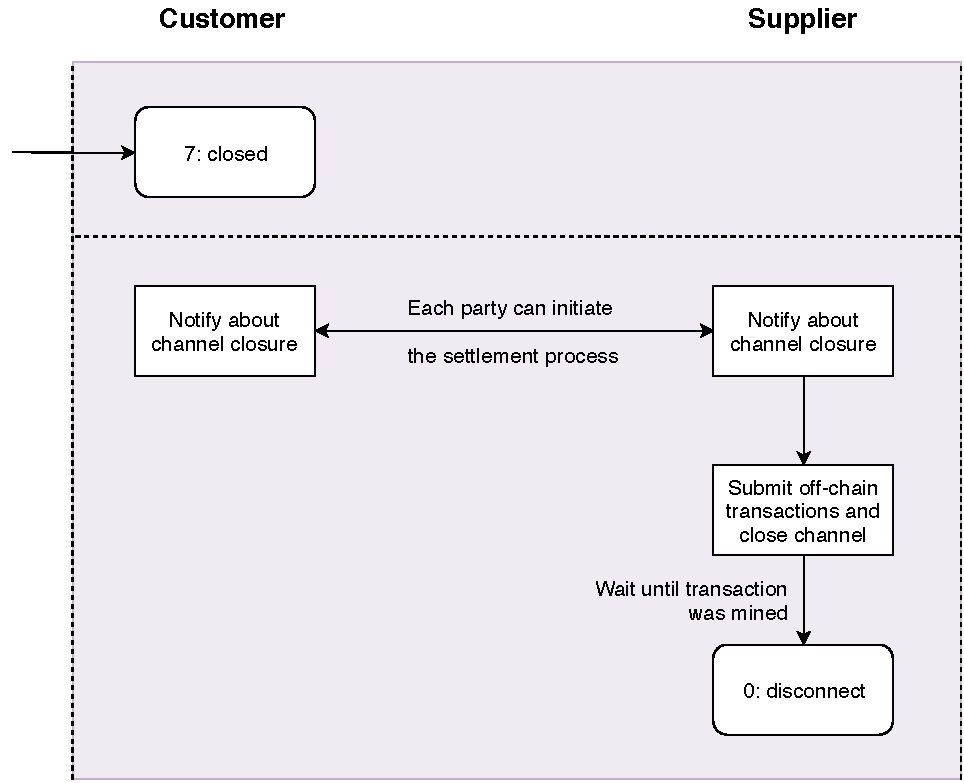
\includegraphics[width=\textwidth]{img/Plug-Socket-settlement_process.pdf}
    \caption{Settlement process}
    \label{fig:settlement_process}
\end{figure}
As soon as a party wants to stop the payment process, e.g. when the battery of the customer is fully charged or the socket received an invalid signature, it can notify the other party about it. The latest valid off-chain transaction, which contains the total value spent by the plug up to this point, is then submitted to the Smart Contract closing the payment channel, in other words settling the transaction on the blockchain. The \textit{closeChannel(uint256 \_value, bytes memory \_signature)} function verifies the submitted signature and pays out the amounts accordingly.
\\
As it is in the interest of the supplier to close the channel with the latest signature, containing the highest value, it’s the sockets task to settle the transaction. The Smart Contract also protects the customer – if the supplier fails to submit a valid signature in a certain amount of time, the deposited amount can be withdrawn again.
\newpage
\subsubsection{Smart Contract}
Security is extraordinarily important for Smart Contract development, as possibly large sums of money are handled and the code is immutable, i.e. can’t be changed once the Smart Contract has been deployed to the Ethereum network. This section will go over the Smart Contract implementation and explain all key functions, some security best practices and design choices. The entire source code can be found under the appendix, listing \ref{lis:safemath} \& \ref{lis:pc_sc}.
\paragraph{SafeMath Library}
Solidity has no built in checks for integer under- and overflows, which can become a major security issue, especially when dealing with balances, allowing an attacker to drain a Smart Contract. A so-called SafeMath library, as the one found under appendix \ref{lis:safemath} can help in preventing integer under- and overflows.
An example on how to use a library for a certain data type can be found in line 70 of the Smart Contract source code:
\begin{lstlisting}[language=Solidity, caption={Using the SafeMath library}, label={lis:safemath_use}, firstnumber=70]
using SafeMath for uint256;
\end{lstlisting}
Here are some examples on how to add, subtract or multiply integers.
\begin{lstlisting}[language=Solidity, caption={Examples for SafeMath calculations}, label={lis:safemath_example}]
uint256 a = 5;
uint256 b = 7;

// add two integers
// c = a + b
uint256 c = a.add(b)

// subtract two integers
// d = b - a
// would result in an integer underflow, therefore the safemath library throws
uint256 d = b.sub(a)

// multiply two integers
// e = a * b
uint256 e = a.mul(b)
\end{lstlisting}
\leavevmode
\\
\paragraph{Off-chain transaction}
As previously mentioned, there is no standard for off-chain transactions and it heavily relies on its implementation. At its core, they are nothing else than a few values that are hashed and signed. The first, most obvious part of the transaction is the value, an unsigned 256 bit integer. The second value is a nonce. It’s necessary to protect the customer against replay attacks. Without the nonce, the supplier could just resubmit an off-chain transaction with a higher value from another payment channel. The nonces are stored in a mapping variable defined in line 96 and initialized with zero for all customers. As soon as a payment channel is closed via the \textit{closeChannel} function in line 148 or the channel times out via the \textit{timeOutChannel} function in line 187, the nonce of the payment channel customer increments by one, rendering all off-chain transactions up to this point invalid for the future. The last value is the contract address, so the transaction is protected against replay attacks on other Smart Contracts.
\\\\
The \textit{verifySignature} function is used to verify the off-chain transaction on the Smart Contract. It takes the value and the signature of the transaction as a parameter. Then in lines 235-241 it takes the 3 values listed above, the value, nonce and contract address and recreates the message used for the signature. First the 3 values are encoded using the \textit{abi.encodePacked()} function and hashed using the \textit{keccak256()} function:
\\
\begin{lstlisting}[language=Solidity, numbers=none]
bytes32 message = keccak256(
  abi.encodePacked(
    _value,
    contractAddress,
    customerNonces[channelCustomer]
  )
);
\end{lstlisting}
\leavevmode
\\
The resulting hash is then prefixed by the Ethereum specific prefix and hashed a second time.
\\
\begin{lstlisting}[language=Solidity, numbers=none]
bytes32 prefixedMessage = keccak256(
  abi.encodePacked(
    "\x19Ethereum Signed Message:\n32",
    message
  )
);
\end{lstlisting}
\leavevmode
\\
This recreates the exact hash that the customer signed to generate the off-chain transaction. With this hash and the signature passed to the function, the sender of the off-chain transaction can be recovered using the \textit{ecrecover} function in line 244 and if it matches the current channel customer stored inside the \textit{channelCustomer} variable in line 91, the function returns true, accepting the off-chain transaction.
\\
\begin{lstlisting}[language=Solidity, numbers=none]
return ecrecover(prefixedMessage, v, r, s) == channelCustomer;
\end{lstlisting}
\leavevmode
\\